% This is a Basic Assignment Paper but with like Code and stuff allowed in it, there is also url, hyperlinks from contents included. 

\documentclass[11pt]{article}

% Preamble

\usepackage[margin=1in]{geometry}
\usepackage{amsfonts, amsmath, amssymb}
\usepackage{fancyhdr, float, graphicx}
\usepackage[utf8]{inputenc} % Required for inputting international characters
\usepackage[T1]{fontenc} % Output font encoding for international characters
\usepackage{fouriernc} % Use the New Century Schoolbook font
\usepackage[nottoc, notlot, notlof]{tocbibind}
\usepackage{listings}
\usepackage{xcolor}
\usepackage{blindtext}
\usepackage{hyperref}
\hypersetup{
    colorlinks=true,
    linkcolor=black,
    filecolor=magenta,      
    urlcolor=cyan,
    pdfpagemode=FullScreen,
    }

\definecolor{codegreen}{rgb}{0,0.6,0}
\definecolor{codegray}{rgb}{0.5,0.5,0.5}
\definecolor{codepurple}{rgb}{0.58,0,0.82}
\definecolor{backcolour}{rgb}{0.95,0.95,0.92}

\lstdefinestyle{mystyle}{
    backgroundcolor=\color{backcolour},   
    commentstyle=\color{codegreen},
    keywordstyle=\color{magenta},
    numberstyle=\tiny\color{codegray},
    stringstyle=\color{codepurple},
    basicstyle=\ttfamily\footnotesize,
    breakatwhitespace=false,         
    breaklines=true,                 
    captionpos=b,                    
    keepspaces=true,                 
    numbers=left,                    
    numbersep=5pt,                  
    showspaces=false,                
    showstringspaces=false,
    showtabs=false,                  
    tabsize=2
}

\lstset{style=mystyle}

% Header and Footer
\pagestyle{fancy}
\fancyhead{}
\fancyfoot{}
\fancyhead[L]{\textit{\Large{Advanced Data Structures - Assignment 3}}}
%\fancyhead[R]{\textit{something}}
\fancyfoot[C]{\thepage}
\renewcommand{\footrulewidth}{1pt}



% Other Doc Editing
% \parindent 0ex
%\renewcommand{\baselinestretch}{1.5}

\begin{document}

\begin{titlepage}
	\centering

	%---------------------------NAMES-------------------------------

	\huge\textsc{
		MIT World Peace University
	}\\

	\vspace{0.75\baselineskip} % space after Uni Name

	\LARGE{
		Advanced Data Structures\\
		Second Year B. Tech, Semester 4
	}

	\vfill % space after Sub Name

	%--------------------------TITLE-------------------------------

	\rule{\textwidth}{1.6pt}\vspace*{-\baselineskip}\vspace*{2pt}
	\rule{\textwidth}{0.6pt}
	\vspace{0.75\baselineskip} % Whitespace above the title



	\huge{\textsc{
			Implementation of Dictionary using Binary Search Tree
		}} \\



	\vspace{0.5\baselineskip} % Whitespace below the title
	\rule{\textwidth}{0.6pt}\vspace*{-\baselineskip}\vspace*{2.8pt}
	\rule{\textwidth}{1.6pt}

	\vspace{1\baselineskip} % Whitespace after the title block

	%--------------------------SUBTITLE --------------------------	

	\LARGE\textsc{
		Assignment No. 3
	} % Subtitle or further description
	\vfill

	%--------------------------AUTHOR-------------------------------

	Prepared By
	\vspace{0.5\baselineskip} % Whitespace before the editors

	\Large{
		Krishnaraj Thadesar \\
		Cyber Security and Forensics\\
		Batch A1, PA 20
	}


	\vspace{0.5\baselineskip} % Whitespace below the editor list
	\today

\end{titlepage}

\tableofcontents
\thispagestyle{empty}
\clearpage

\setcounter{page}{1}

\section{Objectives}
\begin{enumerate}
	\item To study data structure : Binary Search Tree
	\item To study breadth first traversal.
	\item To study different operations on Binary search Tree.
\end{enumerate}

\section{Problem Statement}
Implement dictionary using binary search tree where dictionary stores keywords and its meanings.
Perform following operations:
\begin{enumerate}
	\item Insert a keyword
	\item Delete a keyword
	\item Create mirror image and display level wise
	\item Copy the binary Search Tree
\end{enumerate}

\section{Theory}
\subsection{Binary Search Tree}
\textit{Binary Search Trees are a special type of binary trees where the value of all the nodes in the left sub-tree is less than the value of the root and the value of all the nodes in the right sub-tree is greater than the value of the root.}\\

The left and right sub-trees are also binary search trees. This property of binary search trees makes them useful for searching, as the desired node can be found by repeatedly comparing the input to the value of the root and choosing the appropriate sub-tree, without having to search through the entire tree.

Binary search trees are also useful for sorting, as it is easy to sort the nodes in ascending order by performing an in-order traversal of the tree.

\begin{figure}[H]
	\centering
	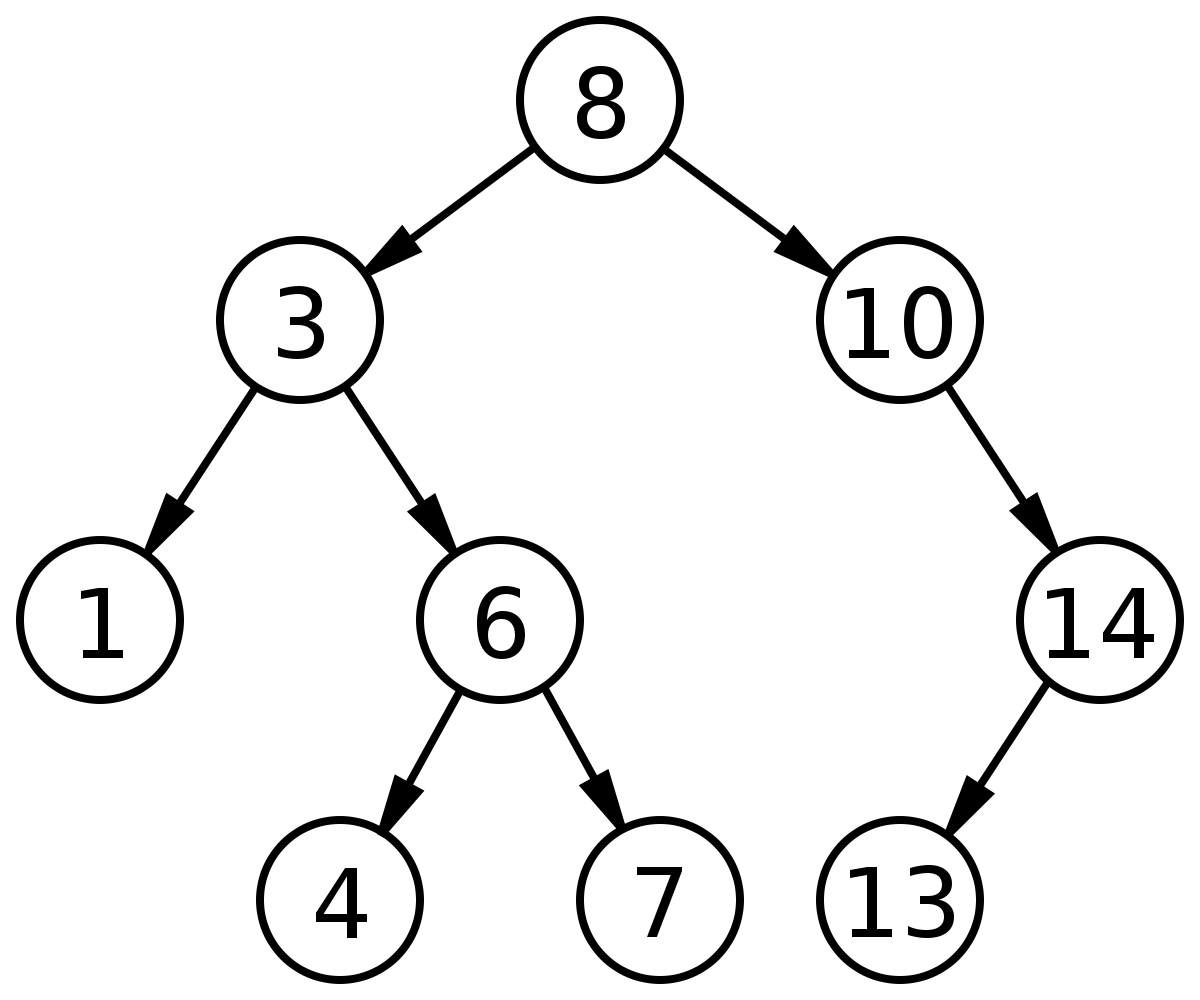
\includegraphics[width=0.30\textwidth]{figures/1200px-Binary_search_tree.svg.png}
	\caption{Example of a Binary Search Tree}
	\label{fig:1200px-Binary_search_tree.svg}
\end{figure}

\subsection{Breadth First Traversal}
Breadth First Traversal (or Level Order Traversal) is a tree traversal algorithm where we should start traversing the tree from root and traverse the tree level wise i.e. traverse the nodes level by level.

In level order traversal, we visit the nodes level by level from left to right.

\subsection{Different operations on binary search tree}

\subsubsection{Copy}
To copy a Binary Search Tree into another Binary Search Tree, we perform a pre-order traversal of the tree. For each node, we create a new node with the same value and then recursively copy the left and right sub-trees of the node.

To copy it Iteratively, we use a queue to store the nodes of the tree. We start by pushing the root node into the queue. We then pop a node from the queue and create a new node with the same value as the popped node. We then push the left and right child of the popped node into the queue and repeat the process until the queue is empty.

\subsubsection{Insert}
To insert a node in a binary search tree, we start by comparing the value of the node to be inserted with the value of the root node. If the value of the node to be inserted is less than the value of the root node, we move to the left sub-tree and repeat the process. If the value of the node to be inserted is greater than the value of the root node, we move to the right sub-tree and repeat the process.

We repeat this process until we reach a leaf node. The new node is then inserted as the left or right child of the leaf node, depending on the value of the node to be inserted.
\subsubsection{Mirror Image}

To create a mirror image of a binary search tree, we perform a pre-order traversal of the tree. For each node, we swap the left and right child of the node. We then recursively create the mirror image of the left and right sub-trees of the node.

To create it Iteratively, we use a stack to store the nodes of the tree. We start by pushing the root node into the stack. We then pop a node from the stack and swap the left and right child of the popped node. We then push the left and right child of the popped node into the stack and repeat the process until the stack is empty.

\begin{figure}[H]
	\centering
	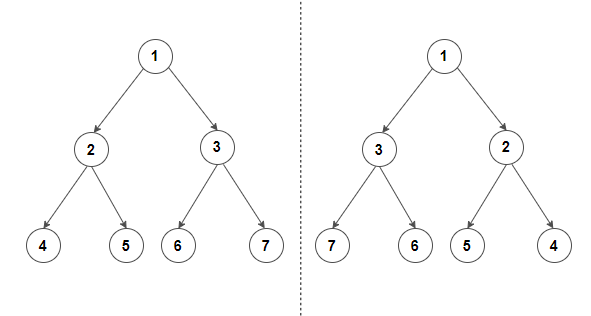
\includegraphics[scale=0.5]{figures/Binary-Tree-Mirror.png}
	\caption{Mirror of a Binary Tree}
	\label{fig:Mirror of a Binary Tree}
\end{figure}


\subsubsection{Delete}

There are 3 Cases for deletion of a node in a binary search tree:

\begin{enumerate}
	\item The node to be deleted is a leaf node. In this case, we simply remove the node from the tree.
	\item The node to be deleted has only one child. In this case, we replace the node to be deleted with its child.
	\item The node to be deleted has two children. In this case, we find the inorder successor of the node. The inorder successor is the smallest node in the right sub-tree of the node. We replace the value of the node to be deleted with the value of the inorder successor. We then delete the inorder successor. The inorder successor will have at most one child node, so we can use the above two cases to delete it.

	      It can also be done using the inorder predecessor. The inorder predecessor is the largest node in the left sub-tree of the node. We replace the value of the node to be deleted with the value of the inorder predecessor. We then delete the inorder predecessor. The inorder predecessor will have at most one child node, so we can use the above two cases to delete it.
\end{enumerate}

\begin{figure}[H]
	\centering
	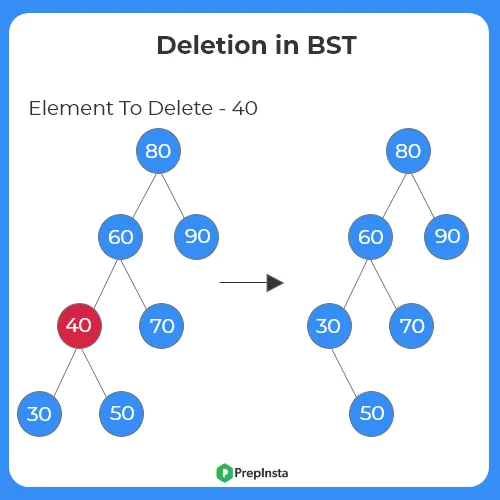
\includegraphics[width=0.45\textwidth]{figures/Deletion_BST.png}
	\caption{Deleting a node from a Binary Search Tree}
	\label{fig:Deleting a node from a Binary Search Tree}
\end{figure}

\section{Platform}
\textbf{Operating System}: Arch Linux x86-64 \\
\textbf{IDEs or Text Editors Used}: Visual Studio Code\\
\textbf{Compilers} : g++ and gcc on linux for C++\\

\section{Input}
\begin{enumerate}
	\item Input at least 10 nodes.
	\item Display binary search tree levelwise traversals of binary search tree with 10 nodes
	\item Display mirror image and copy operations on BST
\end{enumerate}
\section{Output}
\begin{enumerate}
	\item The traversal of the binary tree in different ways.
\end{enumerate}

\section{Test Conditions}
\begin{enumerate}
	\item Input at least 10 nodes.
	\item Display all traversals of binary tree with 10 nodes.(recursive and nonrecursive)
\end{enumerate}

\section{Pseudo Code}
\subsection{Create}
\begin{lstlisting}[language=C++]
	void create_root()
        root = new WordNode
        display - "Enter the data: " << endl
        Take Input of root->word
        Take Input of root->definition
        root->left = NULL
        root->right = NULL
        create_recursive(root)

    void create_recursive(WordNode *Node)
        int choice = 0
        WordNode *new_node
        display - "Enter if you want to enter a left node (1/0): "
             << "for the node -- " << Node->word << ":  " << Node->definition << "-- "
        Take Input of choice
        if (choice == 1)
            new_node = new WordNode
            display - "Enter the data: "
            Take Input of new_node->word
            Take Input of new_node->definition
            Node->left = new_node
            create_recursive(new_node)
        display - "Enter if you want to enter a right node (1/0): "
             << "for the node -- " << Node->word << ":  " << Node->definition << "-- "
        Take Input of choice
        if (choice == 1)
            new_node = new WordNode
            display - "Enter the data: "
            Take Input of new_node->word
            Take Input of new_node->definition
            Node->right = new_node
            create_recursive(new_node)
\end{lstlisting}
\subsection{Display}
\begin{lstlisting}[language=C++]
    void bfs()
    {
        WordNode *temp = root
        queue<WordNode *> q
        q.push(temp)
        while (!q.empty())
        {
            temp = q.front()
            q.pop()
            display - temp->word << " : " << temp->definition << endl
            if (temp->left != NULL)
            {
                q.push(temp->left)
            }
            if (temp->right != NULL)
            {
                q.push(temp->right)
            }
        }
    }
\end{lstlisting}
\subsection{Delete}
\begin{lstlisting}[language=C++]
	void delete_node(WordNode *temp, string word)
    
        WordNode *parent = NULL;
        while (temp != NULL)
            if (temp->word == word)
                break;
            else
                parent = temp;
                if (strcmp(word.c_str(), temp->word.c_str()) < 0)
                    temp = temp->left;
                else
                    temp = temp->right;
        if (temp == NULL)
            Print - "Word not found" - endl;
            return;
        else
            // no child node.
            if (temp->left == NULL && temp->right == NULL)
                if (parent->left == temp)
                    parent->left = NULL;
                else
                    parent->right = NULL;
                delete temp;

			// 1 Child case right.
            else if (temp->left == NULL)
                if (parent->left == temp)
                    parent->left = temp->right;
                else
                    parent->right = temp->right;
                delete temp;

			// 1 Child case left. 
            else if (temp->right == NULL)
                if (parent->left == temp)
                    parent->left = temp->left;
                else
                    parent->right = temp->left;
                delete temp;
            else
                WordNode *temp1 = temp->right;
                while (temp1->left != NULL)
                    temp1 = temp1->left;
                temp->word = temp1->word;
                temp->definition = temp1->definition;
                delete_node(temp->right, temp1->word);
    
\end{lstlisting}
\subsection{Mirror Image}
\begin{lstlisting}[language=C++]
    void mirror_recursive(WordNode *temp)
    {
        if (temp == NULL)
        {
            return
        }
        else
        {
            WordNode *temp1
            // Swapping
            temp1 = temp->left
            temp->left = temp->right
            temp->right = temp1

            // Recursively calling the function
            mirror_recursive(temp->left)
            mirror_recursive(temp->right)
        }
    }
\end{lstlisting}
\subsection{Copy}
\begin{lstlisting}[language=C++]
    WordNode *create_copy_recursive(WordNode *temp)
    {
        if (temp == NULL)
        {
            return NULL
        }
        else
        {
            WordNode *new_node = new WordNode
            new_node->word = temp->word
            new_node->definition = temp->definition
            new_node->left = create_copy_recursive(temp->left)
            new_node->right = create_copy_recursive(temp->right)
            return new_node
        }
    }
\end{lstlisting}

\section{Time Complexity}
\subsection{Create}
\begin{itemize}
	\item \textbf{Time Complexity Worst Case}: \[\bigcirc(n^2)\]
	\item \textbf{Time Complexity Best Case}: \[\bigcirc(\log(n))\]
	      % \item \textbf{Space Complexity}: \[\bigcirc(n^2)\]
\end{itemize}
\subsection{Display}
\begin{itemize}
	\item \textbf{Time Complexity}: \[\bigcirc(n)\]
	      % \item \textbf{Space Complexity}: O(n)
\end{itemize}
\subsection{Delete}
\begin{itemize}
	\item \textbf{Time Complexity}: \[\bigcirc(h)\]\\
	      \[h\] is the height of the Binary search tree.
	      % \item \textbf{Space Complexity}: O(n)
\end{itemize}
\subsection{Mirror Image}
\begin{itemize}
	\item \textbf{Time Complexity}:\[\bigcirc(n)\]
	      % \item \textbf{Space Complexity}: O(n)
\end{itemize}
\subsection{Copy}
\begin{itemize}
	\item \textbf{Time Complexity}:\[\bigcirc(n)\]
	      % \item \textbf{Space Complexity}: O(n)
\end{itemize}

\section{Code}

\subsection{Program}
\lstinputlisting[language=C++]{../Programs/Assignment_3.cpp}

\subsection{Input and Output}
\lstinputlisting[]{../Programs/Assignment_3_output.txt}

\section{Conclusion}
Thus, implemented Dictionary using Binary search tree.
\clearpage

\section{FAQ}
\begin{enumerate}
	\item \textbf{Explain application of BST}\\

	      The Applications of Binary Search Tree are:
	      \begin{enumerate}
		      \item Binary Search Tree is used to implement dictionaries.
		      \item Binary Search Tree is used to implement priority queues.
		      \item Binary Search Tree is used to implement disjoint sets.
		      \item Binary Search Tree is used to implement sorting algorithms.
		      \item Binary Search Tree is used to implement expression trees.
		      \item Binary Search Tree is used to implement Huffman coding.
		      \item Binary Search Tree is used to implement B-trees.
		      \item Binary Search Tree is used to implement red-black trees.
	      \end{enumerate}
	\item \textbf{Explain with example deletion of a node having two child.}\\

	      If a node has two children, then we need to find the inorder successor of the node. The inorder successor is the smallest in the right subtree or the largest in the left subtree. After finding the inorder successor, we copy the contents of the inorder successor to the node and delete the inorder successor. Note that the inorder predecessor can also be used.

	      An Example would be:
	      \begin{verbatim}
    Let us consider the following BST as an example.
          50
         / \
       30   70
       / \  / \
      20 40 60 80
      /  \  / \
    10  25 45 65
\end{verbatim}

	      Deleting 30 will be done in following steps.
	      1. Find inorder successor of 30.
	      2. Copy contents of the inorder successor to 30.
	      3. Delete the inorder successor.
	      4. Since inorder successor is 40 which has no left child, we simply make right child of 30 as the new right child of 20.

	      \begin{verbatim}
             50
            / \
          40   70
          / \  / \
         20 25 60 80
        /     / \
       10     45 65
\end{verbatim}

	\item \textbf{Define skewed binary tree.}\\

	      A binary tree is said to be skewed if all of its nodes have only one child. A skewed binary tree can be either left or right skewed. A left skewed binary tree is a binary tree in which all the nodes have only left child. A right skewed binary tree is a binary tree in which all the nodes have only right child.
\end{enumerate}

\end{document}